%%%%%%%%%%%%%%%%%%%%%%%%%%%%%%%%%%%%%%%%%
% fphw Assignment
% LaTeX Template
% Version 1.0 (27/04/2019)
%
% This template originates from:
% https://www.LaTeXTemplates.com
%
% Authors:
% Class by Felipe Portales-Oliva (f.portales.oliva@gmail.com) with template 
% content and modifications by Vel (vel@LaTeXTemplates.com)
%
% Template (this file) License:
% CC BY-NC-SA 3.0 (http://creativecommons.org/licenses/by-nc-sa/3.0/)
%
%%%%%%%%%%%%%%%%%%%%%%%%%%%%%%%%%%%%%%%%%

%----------------------------------------------------------------------------------------
%	PACKAGES AND OTHER DOCUMENT CONFIGURATIONS
%----------------------------------------------------------------------------------------

\documentclass[
	12pt, % Default font size, values between 10pt-12pt are allowed
	%letterpaper, % Uncomment for US letter paper size
	%spanish, % Uncomment for Spanish
]{fphw}

% Template-specific packages
\usepackage[utf8]{inputenc} % Required for inputting international characters
\usepackage[T1]{fontenc} % Output font encoding for international characters
\usepackage{mathpazo} % Use the Palatino font
\usepackage[dvipsnames]{xcolor}
\usepackage{graphicx} % Required for including images
\usepackage{amsmath}
\usepackage{booktabs} % Required for better horizontal rules in tables
\usepackage{listings} % Required for insertion of code
\usepackage{enumerate} % To modify the enumerate environment
\usepackage{ragged2e}
\usepackage{cancel}
\usepackage{MnSymbol,bbding,pifont}
\usepackage{everyhook}
\usepackage{lscape}
\usepackage{array}
\usepackage{float,graphicx}
\newcommand{\randomcolor}{%
  \definecolor{randomcolor}{RGB}
   {
    \pdfuniformdeviate 256,
    \pdfuniformdeviate 256,
    \pdfuniformdeviate 256
   }%
  \color{randomcolor}%
}

%----------------------------------------------------------------------------------------
%	ASSIGNMENT INFORMATION
%----------------------------------------------------------------------------------------

\title{Assignment \#2} % Assignment title

\author{Luis Alberto Ballado Aradias} % Student name

\date{\today} % Due date

\institute{Centro de Investigación y de Estudios Avanzados del IPN \\ Unidad Tamaulipas} % Institute or school name

\class{Introducción al Análisis de Fourier (Sep - Dec 2022)} % Course or class name

\professor{Dr. Wilfrido Gómez-Flores} % Professor or teacher in charge of the assignment

%----------------------------------------------------------------------------------------


\begin{document}

\maketitle % Output the assignment title, created automatically using the information in the custom commands above

%----------------------------------------------------------------------------------------
%	ASSIGNMENT CONTENT
%----------------------------------------------------------------------------------------

{\color{teal}
  \dotfill
  Transformada de Fourier
\dotfill}

\begin{enumerate}
  \setcounter{enumi}{0}
\item Función 1: \\
  \[f(t) =\left\{ \begin{array}{lr}+1, & -2 < t < -1 \\-1, & 1 < t < 2\\0, & otro\hspace{0.1cm} caso \end{array}\right.\]

  \begin{figure}[H]
    \centering
    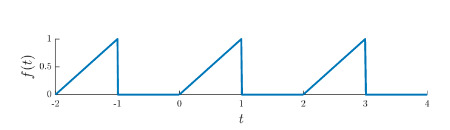
\includegraphics[scale=0.5]{images/funcion_one.jpg}
  \end{figure}
  
\end{enumerate}

$p=\frac{T}{2}=\frac{2}{2}=1$\\
\dotfill
\[a_{0} = \frac{1}{p}\int_{-p}^{p} f(t) \,dt = 1\int_{-1}^{0}0 dt + \int_{0}^{1}t dt =  \frac{t^{2}}{2}\Big|_0^1 = \frac{1}{2} \]
\dotfill
\[a_{n}=\frac{1}{p}\int_{-p}^{p} f(t) cos(\frac{nt\pi}{p}) dt =\]
\[= 1\left[ \int_{-1}^{0} 0*cos(\frac{nt\pi}{1}) dt + \int_{0}^{1} t*cos(\frac{nt\pi}{1}) dt\right]=\]
\[ 1\left[ \int_{0}^{1} t*cos(nt\pi) dt\right]=\]
resolviendo la integral por partes: $u=t$ ; $du=dt$ ; $dv=cos(nt\pi)$ ; $v= \frac{1}{n\pi}sen(nt\pi)$
\[ \frac{t*sen(nt\pi)}{n\pi} \Big|_0^1 - \int \frac{1}{n\pi}*sen(nt\pi) dt =\]
\[ \frac{1}{(n\pi)^{2}} \left[ nt\pi *sen(n\pi) + cos(n\pi) -1 \right] = \]
\[ \frac{cos(n\pi)-1}{(n\pi)^{2}}=\]
\[ a_{n} = \frac{(-1)^{n}-1}{(n\pi)^{2}}\]
\dotfill
\[b_{n}=\frac{1}{p}\int_{-p}^{p} f(t) sen(\frac{nt\pi}{p}) dt =\]
\[= 1\left[ \int_{-1}^{0} 0*sen(\frac{nt\pi}{1}) dt + \int_{0}^{1} t*sen(\frac{nt\pi}{1}) dt\right]=\]
\[ 1\left[ \int_{0}^{1} t*sen(nt\pi) dt\right]=\]
resolviendo la integral por partes: $u=t$ ; $du=dt$ ; $dv=sen(nt\pi)$ ; $v= \frac{-1}{n\pi}cos(nt\pi)$
\[ \frac{-t*cos(nt\pi)}{n\pi} \Big|_0^1 - \int \frac{-1}{n\pi}*cos(nt\pi) dt =\frac{sen(n\pi)-n\pi * cos(n\pi)}{(n\pi)^{2}}= \frac{(-1)^{n}*-n\pi}{(n\pi)^{2}}\]

\newpage
{\color{teal}
\dotfill
Transformada de Fourier
\dotfill}
\begin{figure}[H]
  \centering
  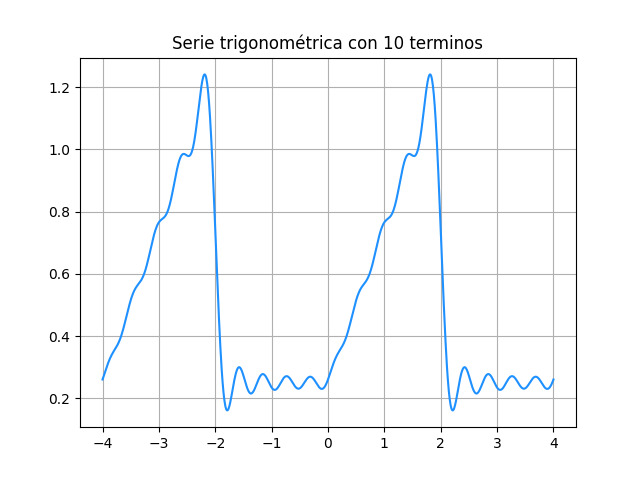
\includegraphics[scale=0.8]{images/funcion1_10.jpg}
\end{figure}

\begin{figure}[H]
  \centering
  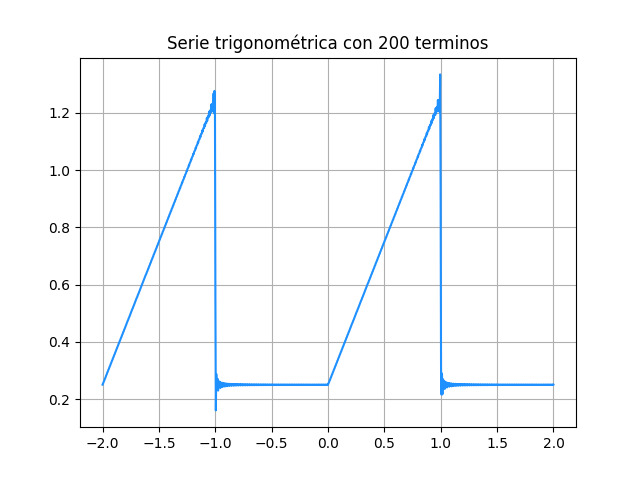
\includegraphics[scale=0.8]{images/funcion1.jpg}
\end{figure}

\newpage
\begin{enumerate}
  \setcounter{enumi}{1}
\item Función 2:

  \[f(t) =\left\{ \begin{array}{lr}t, & 0 < t < 1 \\0, & otro\hspace{0.1cm} caso \end{array}\right.\]
  
  \begin{figure}[H]
    \centering
    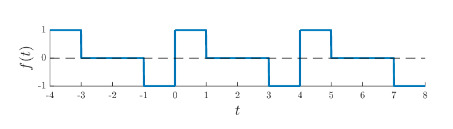
\includegraphics[scale=0.5]{images/funcion_two.jpg}
  \end{figure}
  
\end{enumerate}

$p=\frac{T}{2}=\frac{4}{2}=2$\\
\dotfill
\[a_{0} = \frac{1}{p}\int_{-p}^{p} f(t) \,dt = \frac{1}{2}\int_{-2}^{-1}0 dt + \int_{-1}^{0}-1 dt + \int_{0}^{1}1 dt + \int_{1}^{2}0 dt =  -1+1 = 0 \]
\dotfill
\[a_{n}=\frac{1}{p}\int_{-p}^{p} f(t) cos(\frac{nt\pi}{p}) dt =\]
\[\frac{1}{2}\int_{-2}^{2} f(t) cos(\frac{nt\pi}{2}) dt =\]
\[\frac{1}{2}\int_{-2}^{1} 0*cos(\frac{nt\pi}{2}) dt + \int_{-1}^{0} -1*cos(\frac{nt\pi}{2}) dt + \int_{0}^{1} 1*cos(\frac{nt\pi}{2}) dt + \int_{1}^{2} 0*cos(\frac{nt\pi}{2}) dt =\]
\[ \frac{2*sen(\frac{nt\pi}{2})}{n\pi} - \frac{2*sen(\frac{n\pi}{2})}{n\pi} = 0\]
\dotfill
\[b_{n}=\frac{1}{p}\int_{-p}^{p} f(t) sen(\frac{nt\pi}{p}) dt =\]
\[\frac{1}{2}\int_{-2}^{2} f(t) sen(\frac{nt\pi}{2}) dt =\]
\[\frac{1}{2}\int_{-2}^{1} 0*sen(\frac{nt\pi}{2}) dt + \int_{-1}^{0} -1*sen(\frac{nt\pi}{2}) dt + \int_{0}^{1} 1*sen(\frac{nt\pi}{2}) dt + \int_{1}^{2} 0*sen(\frac{nt\pi}{2}) dt =\]
\[b_{n}=\frac{4*sen^{2}(\frac{n\pi}{4})}{n\pi}\]

\newpage
{\color{teal}
\dotfill
Serie trigonométrica de Fourier
\dotfill}

\begin{figure}[H]
  \centering
  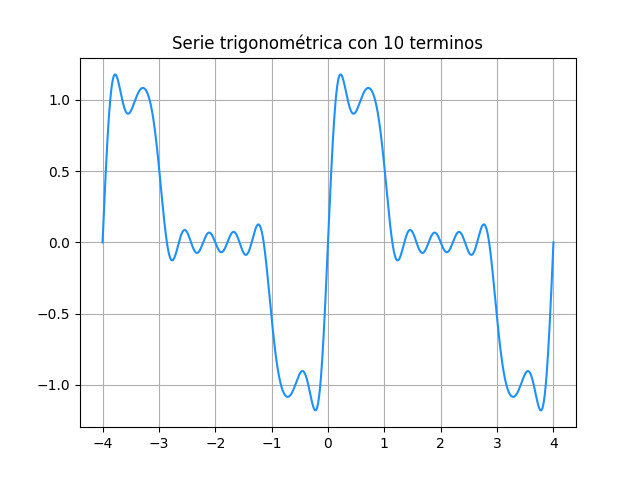
\includegraphics[scale=0.8]{images/funcion3_10.jpg}
\end{figure}

\begin{figure}[H]
  \centering
  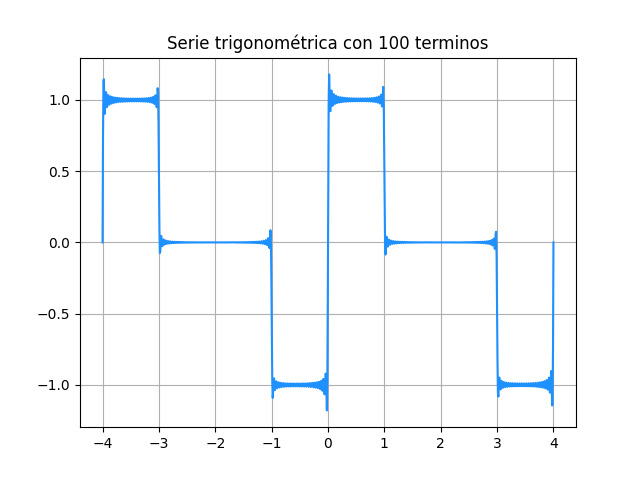
\includegraphics[scale=0.8]{images/funcion3.jpg}
\end{figure}

\newpage
{\color{teal}
\dotfill
Código python
\dotfill}

Con uso de las librerias
\begin{verbatim}
import numpy as np
import math
import matplotlib.pyplot as plt
\end{verbatim}

Coeficiente $a_{n}$
\begin{verbatim}
def an(n):
    n=int(n)
    return (pow(-1,n)-1)/pow(n*np.pi,2) #funcion1
    #return 0 #funcion3
\end{verbatim}

Coeficiente $b_{n}$
\begin{verbatim}
def bn(n):
    n = int(n)
    return ((-n*np.pi)*pow(-1,n))/pow(n*np.pi,2) #funcion1
    #return (4*((math.sin((np.pi*n)/4))**2))/(np.pi*n)#funcion3
\end{verbatim}

Coeficiente $w_{n}$
\begin{verbatim}
def wn(n):
    global T
    wn = (2*np.pi*n)/T
    return wn
\end{verbatim}

Serie de Fourier
\begin{verbatim}
def serie_fourier(armonico,x):

    a0 = 1/2 #funcion1
    #a0 = 0 #funcion3
    sumas = a0

    for n in range(1,armonico):
        try:
            sumas = sumas + an(n)*np.cos(wn(n)*x) + bn(n)*np.sin(wn(n)*x)
        except Exception as e:
            print(e)
            pass
        
    return sumas
\end{verbatim}

%----------------------------------------------------------------------------------------

\end{document}
